\documentclass[varwidth]{standalone}

\usepackage{tikz}
\usepackage{calc}

\pagecolor{yellow!15}
\begin{document}
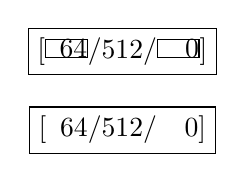
\begin{tikzpicture}

\newlength{\wtmp}
\setlength{\wtmp}{\widthof{589}}

% style: node left pad (for) number (padded with space)
\tikzstyle{nlpn} = [draw=none, align=right, inner sep=0pt, outer sep=0pt, minimum size=0pt, minimum width=\wtmp,text width=\wtmp]

% style for function:    
\tikzstyle{nlpnA} = [nlpn,draw]

% function to insert node:
\def\lpn#1{\tikz\node[nlpnA]{#1};} 

% place node - use function to place node inside
\node[draw] at (0,4) {[\lpn{64}/512/\lpn{0}]};

\tikzstyle{nlpnA} = [nlpn]
\node[draw] at (0,3) {[\lpn{64}/512/\lpn{0}]};

\end{tikzpicture}
\end{document}
